\documentclass[11pt, a4paper]{article}
\usepackage[utf8]{inputenc}
\usepackage{minted}
\usepackage{hyperref}
\usepackage{graphicx}
\graphicspath{{./images/}}

\setlength{\parindent}{0em}
\setlength{\parskip}{1em}

\begin{document}
\title{Concurrency}
\author{Samuel Navarro}
\date{\today}
\maketitle
\tableofcontents{}

\section{Introduction}%
\label{sec:introduction}

Concurrency means that a single system is performing multiple, independent tasks in parallel rather than sequentially as before. Such a system is called a multi-tasking system. 

Multi-tasking does not require multiple processes or multiple cores. Dividing a program execution into many small bits and pieces and by interleaving them with a bits of pieces of other programs we create the illusion of parallelism, which is maintained by the OS. Under the hood we have an extremely fast switching of tasks. 

But true concurrency with tasks that are running at the same time require a parallel architecture. This might mean having multiple processors or multiple cores, or maybe both multiple cores within a processor. This is called \textbf{hardware concurrency.}


An important measure which helps to gauge how many independent tasks can be run in parallel, this is the number of hardware threads on a system. 



\section{Processes and Threads}%
\label{sec:processes_and_threads}



A parallel path of execution is one which runs concurrently with the main program and is thus asynchronous. In contrast to synchronous programs, the main program can continue with its line of execution without the need to wait for the parallel task to complete. The following figure illustrates this difference.




\begin{figure}[htpb!]
	\centering
	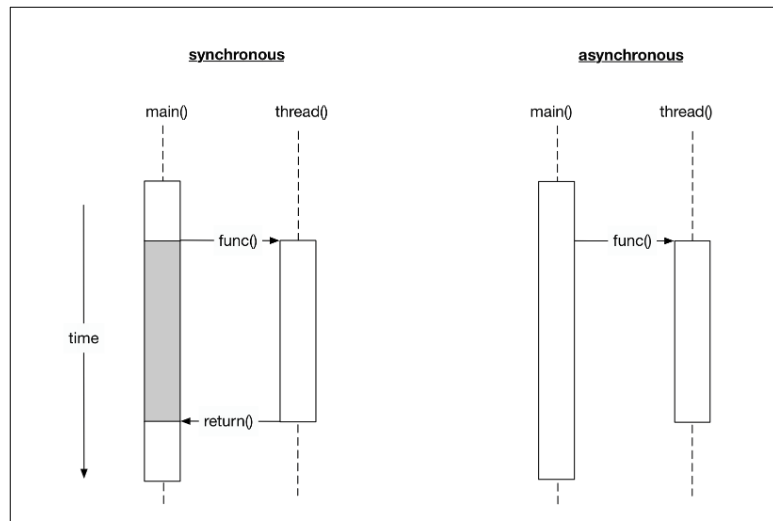
\includegraphics[width=0.8\linewidth]{async_sync}
	\caption{Asynchronous vs Synchronous}
	\label{fig:async_sync}
\end{figure}


A \textbf{process} (also called a \textbf{task}) is a computer program at runtime. It is comprised of the runtime environment provided by the OS, as well as of the embedded binary code of the program during execution. A \textbf{process} is controlled by the OS through certain actions with which it sets the process into one of several carefully defined states:



\begin{figure}[htpb!]
	\centering
	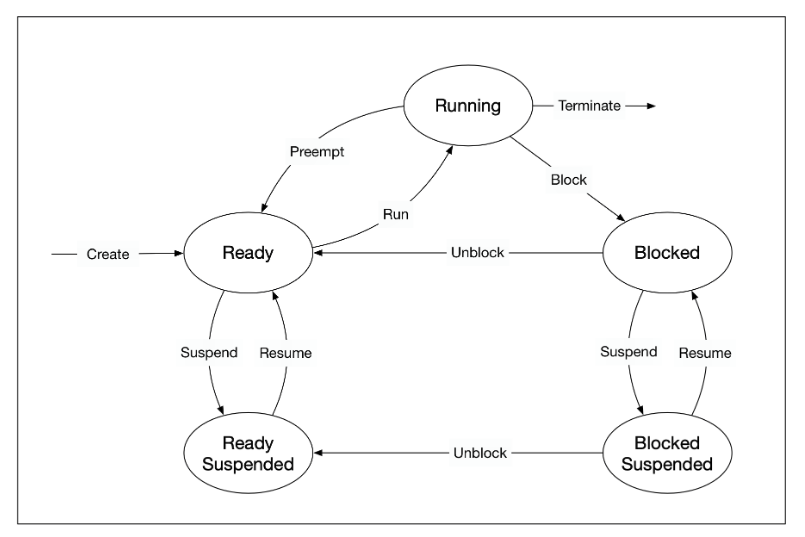
\includegraphics[width=0.8\linewidth]{process}
	\caption{Process}
	\label{fig:process}
\end{figure}


\begin{itemize}
	\item \textbf{Ready} : After its creation, a process enters the ready state and is loaded into main memory. The process now is ready to run and is waiting for CPU time to be executed. Processes that are ready for execution by the CPU are stored in a queue managed by the OS.
	\item \textbf{Running} : The operating system has selected the process for execution and the instructions within the process are executed on one or more of the available CPU cores.
	\item \textbf{Blocked} : A process that is blocked is one that is waiting for an event (such as a system resource becoming available) or the completion of an I/O operation.
	\item \textbf{Terminated} : When a process completes its execution or when it is being explicitly killed, it changes to the "terminated" state. The underlying program is no longer executing, but the process remains in the process table as a "zombie process". When it is finally removed from the process table, its lifetime ends.
	\item \textbf{Ready suspended}: A process that was initially in ready state but has been swapped out of main memory and placed onto external storage is said to be in suspend ready state. The process will transition back to ready state whenever it is moved to main memory again.
	\item \textbf{Blocked suspended} : A process that is blocked may also be swapped out of main memory. It may be swapped back in again under the same conditions as a "ready suspended" process. In such a case, the process will move to the blocked state, and may still be waiting for a resource to become available.
\end{itemize}





Processes are managed by the scheduler of the OS. The scheduler can either let a process run until it ends or blocks (non-interrupting scheduler), or it can ensure that the currently running process is interrupted after a short period of time. The scheduler can switch back and forth between different active processes (interrupting scheduler), alternately assigning them CPU time. The latter is the typical scheduling strategy of any modern operating system.

Since the administration of processes is computationally taxing, operating systems support a more resource-friendly way of realizing concurrent operations: the threads.


A \textit{thread} represents a concurrent execution unit within a process. In contrast to full-blown processes as described above, threads are characterized as light-weight processes (LWP). There are significantly easier to create and destroy: In many systems the creation of a thread is up to 100 times faster than the creation of a process. This is especially advantageous in situations, when the need for concurrent operations changes dynamically. 


\begin{figure}[htpb!]
	\centering
	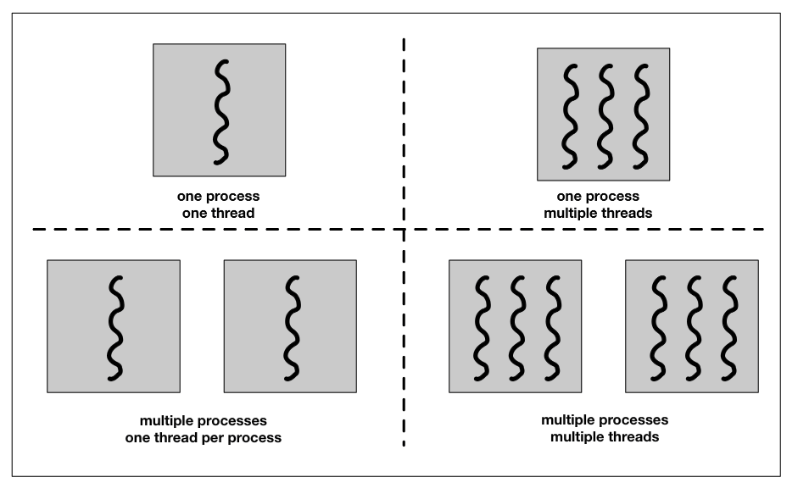
\includegraphics[width=0.8\linewidth]{process_threads}
	\caption{Process and Threads}
	\label{fig:process_threads}
\end{figure}




Threads exist within processes and share their resources. As illustrated by the Figure~\ref{fig:process_threads}, a process can contain several threads or - if no parallel processing is provided for in the program flow - only a single thread.

A major difference between a process and a thread is that each process has its own address space, while a thread does not require a new address space to be created. All the threads in a process can access its shared memory. Threads also share other OS dependent resources such as processors, files, and network connections. As a result, the management overhead for threads is typically less than for processes. Threads, however, are not protected against each other and must carefully synchronize when accessing the shared process resources to avoid conflicts.


Similar to processes, threads exist in different states, which are illustrated in the Figure~\ref{fig:threads}: 


\begin{figure}[htpb!]
	\centering
	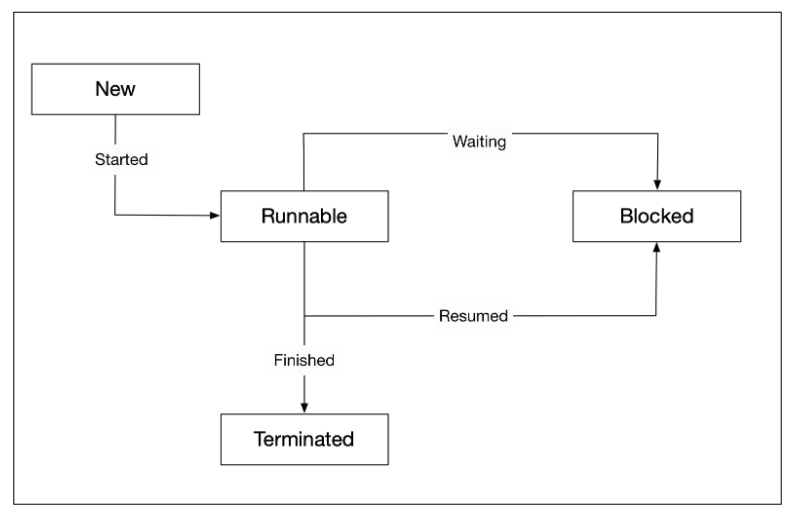
\includegraphics[width=0.8\linewidth]{threads}
	\caption{Threads}
	\label{fig:threads}
\end{figure}


\begin{itemize}
	\item \textbf{New} : A thread is in this state once it has been created. Until it is actually running, it will not take any CPU resources.
	\item \textbf{Runnable} : In this state, a thread might actually be running or it might be ready to run at any instant of time. It is the responsibility of the thread scheduler to assign CPU time to the thread.
	\item \textbf{Blocked} : A thread might be in this state, when it is waiting for I/O operations to complete. When blocked, a thread cannot continue its execution any further until it is moved to the runnable state again. It will not consume any CPU time in this state. The thread scheduler is responsible for reactivating the thread.
\end{itemize}




\begin{itemize}
	\item In a concurrent program, \textbf{threads} share memory. Thus, many \textbf{threads} can access and modify the same memory.
	\item Creating a \textbf{process} is fairly resource-intensive. It is generally more efficient to use several \textbf{threads} within a \textbf{process}.
	\item In contrast to a \textbf{process}, \textbf{threads} are characterized as light-weight. They are significantly easier to create and destroy.
	\item Inter-thread communication can be faster than inter-process communication.
\end{itemize}


\section{Starting a Second Thread}%
\label{sec:starting_a_second_thread}



If we want to start a second thread in addition to the main thread of our program, we need to construct a thread object and pass it the function we want to be executed by the thread. Once the thread enters the runnable state, the execution of the associated thread function may start at any point in time.

\texttt{std::thread t (threadFunction);} 


After the thread object has been constructed, the main thread will continue and execute the remaining instructions until it reaches the end and returns. It is possible that by this point in time, the thread will also have finished. But if this is not the case, the main program will terminate and the resources of the associated process will be freed by the OS. As the thread exists within the process, it can no longer access those resources and thus not finish its execution as intended.

To prevent this from happening and have the main program wait for the thread to finish the execution of the thread function, we need to call \texttt{join()} on the thread object. This call will only return when the thread reaches the end of the thread function and block the main thread until then.  

An example of this is in the file \texttt{main\_and\_sec\_threads.cpp}


\subsection{Randomness of events}%
\label{sub:randomness_of_events}

One very important trait of concurrent programs is their non-deterministic behavior. It can not be predicted which thread the scheduler will execute at which point in time. In the code on \texttt{randomness\_of\_events.cpp}, the amount of work to be performed both in the thread function and in main has been split into two separate jobs. The output in the console differs. 


\textbf{We can use \texttt{join()} as a barrier}

Because the order of execution is determined by the scheduler, if we wanted to ensure that the thread function completed its work before the main function started its own work \textbf{(because it might be waiting for a result to be available)}, we could achieve this by repositioning the call to join.


In the file, the \texttt{.join()} can be moved to before the work in \texttt{main()}. The order of execution now always looks the same.


\subsection{Detach}%
\label{sub:detach}



Let us now take a look at what happens if we don’t join a thread before its destructor is called. When we comment out join in the example above and then run the program again, it aborts with an error. The reason why this is done is that the designers of the C++ standard wanted to make debugging a multi-threaded program easier: Having the program crash forces the programmer to remember joining the threads that are created in a proper way. Such a hard error is usually much easier to detect than soft errors that do not show themselves so obviously.

There are some situations however, where it might make sense to not wait for a thread to finish its work. This can be achieved by "detaching" the thread, by which the internal state variable "joinable" is set to "false". This works by calling the \texttt{detach()} method on the thread. \textbf{The destructor of a detached thread does nothing: It neither blocks nor does it terminate the thread}. In the following example, detach is called on the thread object, which causes the main thread to immediately continue until it reaches the end of the program code and returns. Note that a detached thread can not be joined ever again.


Programmers should be very careful though when using the \texttt{detach()} method. You have to make sure that the thread does not access any data that might get out of scope or be deleted. Also, we do not want our program to terminate with threads still running. Should this happen, such threads will be terminated very harshly without giving them the chance to properly clean up their resources - what would usually happen in the destructor. So a well-designed program usually has a well-designed mechanism for joining all threads before exiting.





\section{Starting a Thread with a Function Object}%
\label{sec:starting_a_thread_with_a_function_object}

We now want to pass a function object instance to the thread. This is basically an instance of a class that implements the function call operator. This can be very useful to passing data through threads. Another way to pass data and also start a thread with a very small code footprint is to use a so-called Lambda function. 



Passing functions to other functions is one form of a \textit{callable object}.

In C++, callable objects are objects that can appear as the left-hand operand of the call operator. These can be pointers to functions, objects of a class that defines an overloaded function call operator and \textit{lambdas}, with which function objects can be created in a very simple way. In the context of \textbf{concurrency}, we can use callable objects to attach a function to a thread. 

In the Section~\ref{sec:starting_a_second_thread} we constructed a thread object by passing a function to it without any arguments. If we were limited to this approach, the only way to make data available from within the thread function would be to use global variables - \textit{which is definitely not recommendable and also incredibly messy.}





The extra parenthesis in the file \texttt{mostVexingParse} is known as C++'s \textit{most vexing parse}, which is a specific form of syntactic ambiguity resolution in the C++ programming language.

The \textit{"most vexing parse"} comes from a rule in C++ that says that anything that could be considered as a function declaration, the compiler should parse it as a function declaration - even if it could be interpreted as something else.


The line:

\texttt{std::thread t(Vehicle());} 

is seemingly ambiguous, since it could be interpreted either as:

\begin{enumerate}
	\item a variable definition for variable t of class \texttt{std::thread}, initialized with an anonymous instance of class Vehicle, or
	\item a function declaration for a function t that return an object of type \texttt{std::thread}  and has a single (unnamed) parameter that is a pointer to function returning an object of type Vehicle.
\end{enumerate}


Most programmers would presumable expect the first case to be true, but the C++ standard requires it to be interpreted as the second - hence the compiler warning. 


There are three ways of forcing the compiler to consider the line as the first case, which would create the thread object we want:


\begin{itemize}
  \item Add an extra pair of parentheses: \texttt{std::thread t1 ( (Vehicle()) );} 
	\item Use copy initialization. \texttt{std::thread t2 = std::thread( Vehicle() ) ;} 
	\item Use uniform initialization with braces. \texttt{std::thread t3\{Vehicle()\};} 
\end{itemize}

Whichever option we use, the idea is the same: the function object is copied into internal storage accessible to the new thread, and the new thread invokes the operator \texttt{()}. Th \texttt{Vehicle()} class can of course have data members and other member functions too, and this is one way of passing data to the thread function: pass it in as a constructor argument and store it as a data member.

File: \texttt{PassingDataToThread.cpp} 




\subsection{Lambdas}%
\label{sub:lambdas}


Another useful way of starting a thread and passing information to it is by using a lambda expression. C++ Lambdas have the properties of being unnamed and capturing variables from the surrounding context, but lack the ability to execute and return functions. 

A Lambda is often used as an argument for functions that can take a callable object. A Lambda is a function object, so it has a type and can be stored and passed around. Its result object is called a \textit{"closure"}, which can be called using the operator \texttt{()} 

It formally consists of three parts: a capture list \texttt{[]}, a parameter list \texttt{()} and a main part \texttt{\{\}}, which contains the code to be executed when the lambda is called. Note that in principal all parts could be empty.

The capture list \texttt{[]}: By default, variables outside of the enclosing {} around the main part of the Lambda can not be accessed. By adding a variable to the capture list however, it becomes available within the Lambda \textbf{either as a copy or as a reference}. The captured variables become a part of the Lambda.

By default, variables in the capture block can not be modified within the Lambda. Using the keyword "mutable" allows to modify the parameters captured by copy, and to call their non-const member functions within the body of the Lambda.


Even though we have been using Lambdas in the above example in various ways, it is important to note that a Lambda does not exist at runtime. The runtime effect of a Lambda is the generation of an object, which is known as closure. The difference between a Lambda and the corresponding closure is similar to the distinction between a class and an instance of the class. A class exists only in the source code while the objects created from it exist at runtime.

We can use (a copy of) the closure (i.e. f0, f1, …) to execute the code within the Lambda at a position in our program different to the line where the function object was created.

The parameter list () : The way parameters are passed to a Lambda is basically identical to calling a regular function. If the Lambda takes no arguments, these parentheses can be omitted (except when "mutable" is used).



\textbf{Question} What's the difference between capture list and parameter list. See this \href{https://stackoverflow.com/questions/28669941/c-lambdas-capture-list-vs-parameter-list}{link}

It seems that the capture list is to keep a state.


\begin{listing}
\begin{minted}[linenos,numbersep=5pt,frame=lines,framesep=2mm]{cpp}
#include <iostream>

int main(){
	const auto addSome = [](double some){
		return [some](double val){ return some + val;};
	};


	const auto addFive = addSome(5);

	std::cout << addFive(2) << std::endl;
	std::cout << addFive(3) << std::endl;
	/*
  OUTPUT:
  7
	8
	* */
	return 0;
}
\end{minted}
\caption{Capture vs Parameter List in Lambda Functions}
\label{lst:capture_vs_parameter_list_in_lambda_functions}
\end{listing}









Let's say we have this code snippet:




\begin{listing}
\begin{minted}[linenos,numbersep=5pt,frame=lines,framesep=2mm]{cpp}
#include <iostream>

int main()
{
    int id = 0; // Define an integer variable

    // capture by reference (immutable)
    auto f0 = [&id]() { std::cout << "a) ID in Lambda = " << id << std::endl; };

    // capture by value (mutable)
    auto f1 = [id]() mutable { std::cout << "b) ID in Lambda = " << ++id << std::endl; };
    f1(); // call the closure and execute the code witin the Lambda
    std::cout << "c) ID in Main = " << id << std::endl;

    // capture by reference (mutable)
    auto f2 = [&id]() mutable { std::cout << "d) ID in Lambda = " << ++id << std::endl; };
    f2(); 
    std::cout << "e) ID in Main = " << id << std::endl; 

    // pass parameter 
    auto f3 = [](const int id) { std::cout << "f) ID in Lambda = " << id << std::endl; };   
		//Before we pass id into it, we increase it by one.
		//That's why we have id = 2
    f3(++id);

    // observe the effect of capturing by reference at an earlier point in time
		// Because we pass by reference the id, we have Id=2
    f0(); 

    return 0;
}
\end{minted}
\caption{Capture Variables by Value and Reference}
\label{lst:capture_variables_by_value_and_reference}
\end{listing}


Pass by value means that we are going to make a copy of the parameter; we're not going to change the original ID. But, because the lambda is \texttt{mutable} that means that ID can be change within the Lambda itself. 


In Listing~\ref{lst:capture_variables_by_value_and_reference}. The output will be:
\begin{itemize}
	\item b) ID lambda = 1
	\item c) ID Main = 0
	\item d) ID lambda = 1
	\item e) ID Main = 1
	\item f) ID lambda = 2
	\item a) Id lambda = 2
\end{itemize}





Another example is in file: \texttt{startThreadsLambdas.cpp}. Here, the output in the main thread is generated first, at which point the variable ID has taken the value 1. Then, the call-by-value thread is executed with ID at a value of 0. Then, the call-by-reference thread is executed with ID at a value of 1. This illustrates the effect of passing a value by reference : when the data to which the reference refers changes before the thread is executed, those changes will be visible to the thread. We will see other examples of such behavior later in the course, as this is a primary source of concurrency bugs.


Intuition: The lambda which passes by value the id, gets id = 0. Also, the pass by reference function gets id=0, but, by the time the function finishes its work, id now has turned into 1.






\section{Starting a Thread with Variadic Templates and Member Functions}%
\label{sec:starting_a_thread_with_variadic_templates_and_member_functions}


\textbf{Variadic Templates}: They allow the definition of functions that take a varying number of arguments which is handy in concurrency because we can use them to pass several arguments to a thread. 

\textbf{Member Functions} We can pass arguments to a thread by reference, but what if we wish to run a function other than the function call operator. We want to run functions of already existent objects. 



We have seen that one way to pass arguments in to the thread function is to package them in a class using the function call operator. Even though this worked well, it would be very cumbersome to write a special class every time we need to pass data to a thread. We can also use a Lambda that captures the arguments and then calls the function. But there is a simpler way: The thread constructor may be called with a function and all its arguments. That is possible because the thread constructor is a \textit{variadic template} that takes multiple arguments.


\subsection{Variadic Templates}%
\label{sub:variadic_templates}



The need for \textbf{variadic templates} could be illustrated in the Listing~\ref{lst:variadic_templates}. The second thread object is constructed with a function \texttt{printIDAndName}, which requires an int and a string, but if we only pass a single argument to the thread when calling\texttt{printIDAndName} a compiler error will occur.  



\begin{listing}
\begin{minted}[linenos,numbersep=5pt,frame=lines,framesep=2mm]{cpp}
#include <iostream>
#include <thread>
#include <string>

void printID(int id)
{
    std::this_thread::sleep_for(std::chrono::milliseconds(50));
    std::cout << "ID = " << id << std::endl;
    
}

void printIDAndName(int id, std::string name)
{
    std::this_thread::sleep_for(std::chrono::milliseconds(100));
    std::cout << "ID = " << id << ", name = " << name << std::endl;
}

int main()
{
    int id = 0; // Define an integer variable

    // starting threads using variadic templates
    std::thread t1(printID, id);
    std::thread t2(printIDAndName, ++id, "MyString");
    std::thread t3(printIDAndName, ++id); // this procudes a compiler error

    // wait for threads before returning
    t1.join();
    t2.join();
    //t3.join();


    return 0;
}
\end{minted}
\caption{Variadic Templates}
\label{lst:variadic_templates}
\end{listing}




There is one more difference between calling a function directly and passing it to a thread: With the former, arguments may be passed by value, by reference or by using move semantics - depending on the signature of the function. When calling a function using a variadic template, the arguments are by default either moved or copied - depending on wether they are rvalues or lvalues. There are ways however which allow us to overwrite this behavior. If you want to move an lvalue for example, we can call std::move. 


In the file \texttt{MoveVsCopybyValue.cpp}, two threads are started. One where the string is \textbf{copied by value}. This allows us to print name1 even after \texttt{join} has been called. The second one is passed to the thread function using \textbf{move semantics}, which means that it is not available any more after \texttt{join} has been called.


In the file \texttt{PassDataAsRef.cpp}, when passing the string variable name to the thread funciton, we need to explicity mark it as a reference, so the compiler threat it as such. This is done using \texttt{std::ref}.


Even though the code works, we are now sharing mutable data between threads - \textbf{which is a primary source for concurrency bugs.}

\subsection{Starting Threads with Member Functions}%
\label{sub:starting_threads_with_member_functions}



What if we want to run a member function other than the function call operator, such as a member function of an existing object?. In C++, for calling member functions, the \texttt{std::thread} function requires an additional argument for the object on which to invoke the member function.


In the \texttt{ThreadsMemberFunc.cpp}, the Vehicle object v1 is passed to the thread function by value, thus a copy is made which does not affect the \textit{original} living in the main thread. That's why changes to its members variable \texttt{\_id} will thus not show when printing later in main. 

In the second Vehicle object, because it's passed by reference, changes to its \texttt{\_id} variable will also be visible in the main thread. 


Another thing to consider is that we have to ensure that the existence of \texttt{v2} outlives the completion of the thread \texttt{t2} - otherwise there will be an attempt to access an invalidated memory address. An alternative is to use a heap-allocated object and a reference-counted pointer such as \texttt{std::shared\_ptr<Vehicle>} to ensure that the object lives as long as it takes the thread to finish its work. The file 



\section{Running Multiple Threads}%
\label{sec:running_multiple_threads}


\subsection{Fork-Join Parallelism}%
\label{sub:fork_join_parallelism}

The basic mechanism of this concept follows a simple three-step pattern:

\begin{enumerate}
	\item Split the flow of execution into a parallel thread ( \textit{"fork"})
	\item Perform some work in both the main thread and the parallel thread.
	\item Wait for the parallel thread to finish and unite the the split flow of execution again \textit{("join")}.
\end{enumerate}





\begin{figure}[htpb!]
	\centering
	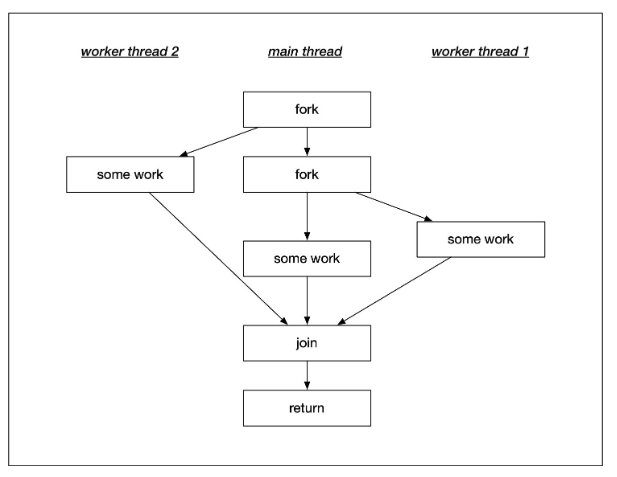
\includegraphics[width=0.8\linewidth]{fork_join}
	\caption{Fork-Join Parallelism}
	\label{fig:fork_join_parallelism}
\end{figure}


In the main thread, the program flow is forked into three parallel branches. In both worker branches, some work is performed - which is why threads are often referred to as \textit{"worker threads"}. Once the work is completed, the flow of execution is united again in the main function using the \texttt{join()}  command. In this example, join acts as a barrier where all threads are united. The execution of main is in fact halted, until both worker threads have successfully completed their respective work. 



In the \texttt{forkJoinParallelism.cpp} file, if we try to compile the program using the \texttt{push\_back()} function, we get a compiler error. The problem with our code is that by pushing the thread object into the vector, we attempt to make a copy of it. However, thread objects do not have a copy constructor and thus can not be duplicated. If this were possible, we would create yet another branch in the flow of execution - which is not what we want. The solution to this problem is to use move semantics, which provide a convenient way for the contents of objects to be 'moved' between objects, rather than copied. It might be a good idea at this point to refresh your knowledge on move semantics, on rvalues and lvalues as well as on rvalue references, as we will make use of these concepts throughout the course.

To solve our problem, we can use the function \texttt{emplace\_back()} instead of \texttt{push\_back()} which internally uses move semantics to move our thread object into the vector without making a copy. 

The console output is really messy. the components are completely intermingled. Also, when the program is run several times, the output will look different with each execution.


\begin{itemize}
	\item The order in which threads are executed is non-deterministic. Every time a program is executed, there is a chance for a completely different order of execution.
	\item Threads may get preempted in the middle of execution and another thread may be selected to run.
\end{itemize}


\textbf{These two properties pose a major problem with concurrent applications: A program may run correctly for thousands of times and suddenly, due to a particular interleaving of threads, there might be a problem. From a debugging perspective, such errors are very hard to detect as they can not be reproduced easily.}





In the file \textbf{properMultipleThreads.cpp}: the bug comes from accessing a shared memory location. (Remember that the lambda function in the code used \texttt{id}  by reference. 













\end{document}
